\documentclass[aspectratio=169]{beamer}

\usetheme{Madrid}
\usecolortheme{default}
\setbeamertemplate{navigation symbols}{}
\usepackage{eso-pic}
\usepackage[brazil]{babel}
\shorthandoff{"}
\usepackage[T1]{fontenc}
\usepackage[utf8]{inputenc}
\usepackage{lmodern}

\usepackage{tikz}
\usetikzlibrary{arrows.meta, positioning, shapes.geometric, fit, calc, backgrounds}
\usepackage{listings}
\usepackage{xcolor}

\definecolor{meuazul}{RGB}{0, 79, 151}
\definecolor{meucinza}{RGB}{80, 80, 80}
\definecolor{meuvermelhoescuro}{RGB}{180, 30, 30}
\definecolor{meuverde}{RGB}{30, 130, 60}
\setbeamercolor{structure}{fg=meuazul}

\title[Resposta a Emergências]{Resposta a Emergências}
\subtitle{Engenharia da Qualidade e Confiabilidade}
\author{Prof. Me. Sergio Souza Novak — UniRV}
\titlegraphic{
\includegraphics[width=2cm]{logo.png}}

\begin{document}

% Slide de Título
\frame[plain]{\titlepage}

\AddToShipoutPictureFG{
    \put(\LenToUnit{.92\paperwidth},\LenToUnit{.185\paperheight})
    {\vtop{{\null}\makebox{
\includegraphics[width=.8cm,keepaspectratio]{logo.png}}}}}

% ----------------------------------------------------------------
% SLIDE 1 — MTTF e MTTR
% ----------------------------------------------------------------
\begin{frame}{1) Confiabilidade: MTTF e MTTR}

  \begin{columns}[T]
    \column{0.46\textwidth}
      \textbf{Métricas fundamentais:}
      \begin{itemize}
        \item \textbf{MTTF} — Mean Time To Failure\\
              \textit{Tempo médio até a próxima falha}
        \item \textbf{MTTR} — Mean Time To Repair\\
              \textit{Tempo médio para recuperação}
        \item \textbf{Disponibilidade} depende de ambos:
        \[
          A = \frac{\text{MTTF}}{\text{MTTF} + \text{MTTR}}
        \]
        \item A métrica \textbf{mais crítica} na resposta a emergências é o \textbf{MTTR}
      \end{itemize}

    \column{0.50\textwidth}
      \centering
      \begin{tikzpicture}[font=\small, scale=0.85, transform shape]
        % Linha do tempo
        \draw[->, thick, meuazul] (0,0) -- (8.2,0) node[right] {tempo};

        % Falha 1
        \draw[thick, meuverde] (0,0.1) -- (2.5,0.1);
        \draw[thick, meuvermelhoescuro] (2.5,0.1) -- (3.5,0.1);
        % Falha 2
        \draw[thick, meuverde] (3.5,0.1) -- (6.5,0.1);
        \draw[thick, meuvermelhoescuro] (6.5,0.1) -- (7.5,0.1);

        % Setas MTTF
        \draw[<->, thick, meuverde] (0,0.7) -- (2.5,0.7)
          node[midway, above] {\textcolor{meuverde}{MTTF}};
        \draw[<->, thick, meuverde] (3.5,0.7) -- (6.5,0.7)
          node[midway, above] {\textcolor{meuverde}{MTTF}};

        % Setas MTTR
        \draw[<->, thick, meuvermelhoescuro] (2.5,-0.5) -- (3.5,-0.5)
          node[midway, below] {\textcolor{meuvermelhoescuro}{MTTR}};
        \draw[<->, thick, meuvermelhoescuro] (6.5,-0.5) -- (7.5,-0.5)
          node[midway, below] {\textcolor{meuvermelhoescuro}{MTTR}};

        % Marcadores
        \foreach \x in {0, 2.5, 3.5, 6.5, 7.5}
          \draw[thick] (\x, -0.15) -- (\x, 0.15);

        % Legenda
        \node[meuverde, right] at (0,-1.2) {{\tiny $\blacksquare$} Sistema operacional};
        \node[meuvermelhoescuro, right] at (0,-1.7) {{\tiny $\blacksquare$} Em reparo};
      \end{tikzpicture}
  \end{columns}
\end{frame}

% ----------------------------------------------------------------
% SLIDE 2 — Latência Humana
% ----------------------------------------------------------------
\begin{frame}{2) Seres Humanos Acrescentam Latência}

  \begin{columns}[T]
    \column{0.46\textwidth}
      \begin{itemize}
        \item Humanos introduzem \textbf{atrasos} no processo de recuperação:
          \begin{itemize}
            \item Detecção do alerta
            \item Avaliação do problema
            \item Tomada de decisão
            \item Execução da ação
          \end{itemize}
        \item \textbf{Sistemas automatizados} respondem em milissegundos
        \item Um sistema com \textbf{mais falhas}, mas com recuperação automática, pode ter \textbf{maior disponibilidade} que um sistema mais estável, porém dependente de intervenção manual
      \end{itemize}

    \column{0.50\textwidth}
      \centering
      \begin{tikzpicture}[font=\small, node distance=0.9cm and 1.6cm,
                          every node/.style={align=center}]
        \tikzstyle{caixa}=[rectangle, rounded corners=4pt, draw, thick,
                           minimum width=2.6cm, minimum height=0.7cm,
                           fill=blue!10, draw=meuazul]
        \tikzstyle{seta}=[->, thick, meuazul]

        \node[caixa] (alerta) {Alerta disparado};
        \node[caixa, below=of alerta] (detec) {Detecção humana};
        \node[caixa, below=of detec] (aval) {Avaliação};
        \node[caixa, below=of aval] (acao) {Ação corretiva};
        \node[caixa, below=of acao, fill=green!15, draw=meuverde]
              (ok) {Sistema saudável};

        \draw[seta] (alerta) -- (detec)
          node[midway, right, font=\scriptsize, meucinza] {~minutos};
        \draw[seta] (detec) -- (aval)
          node[midway, right, font=\scriptsize, meucinza] {~minutos};
        \draw[seta] (aval) -- (acao)
          node[midway, right, font=\scriptsize, meucinza] {~minutos};
        \draw[seta] (acao) -- (ok);
      \end{tikzpicture}
  \end{columns}
\end{frame}

% ----------------------------------------------------------------
% SLIDE 3 — Manual de Regras (Runbook)
% ----------------------------------------------------------------
\begin{frame}{3) O Manual de Regras (\textit{Runbook})}

  \begin{columns}[T]
    \column{0.50\textwidth}
      \begin{itemize}
        \item Registrar boas práticas \textbf{com antecedência} reduz o MTTR em até \textbf{3$\times$}
        \item \textbf{Improvisar} durante uma crise é arriscado e lento
        \item O \textit{runbook} deve conter:
          \begin{itemize}
            \item Passos claros e ordenados
            \item Critérios de diagnóstico
            \item Comandos prontos para uso
            \item Escalonamento de responsabilidades
          \end{itemize}
        \item \textbf{Engenheiro treinado + runbook} supera o ``herói'' improvisado
      \end{itemize}

    \column{0.46\textwidth}
      \centering
      \begin{tikzpicture}[font=\small, scale=0.9, transform shape]
        \tikzstyle{caixa}=[rectangle, rounded corners=4pt, draw=meuazul, thick,
                           fill=blue!10, minimum width=3.0cm, minimum height=0.65cm,
                           text centered]

        % Sem runbook
        \node[caixa, fill=red!15, draw=meuvermelhoescuro] (sem) at (0,0)
          {Sem Runbook};
        \node[caixa, fill=red!10, draw=meuvermelhoescuro] (imp) at (0,-1)
          {Improviso};
        \node[caixa, fill=red!10, draw=meuvermelhoescuro] (mttr3) at (0,-2)
          {MTTR: $3\times$ maior};

        % Com runbook
        \node[caixa, fill=green!15, draw=meuverde] (com) at (4.0,0)
          {Com Runbook};
        \node[caixa, fill=green!10, draw=meuverde] (proc) at (4.0,-1)
          {Processo definido};
        \node[caixa, fill=green!10, draw=meuverde] (mttr1) at (4.0,-2)
          {MTTR: referência};

        \draw[->, thick, meuvermelhoescuro] (sem) -- (imp);
        \draw[->, thick, meuvermelhoescuro] (imp) -- (mttr3);
        \draw[->, thick, meuverde] (com) -- (proc);
        \draw[->, thick, meuverde] (proc) -- (mttr1);

        % Vs
        \node[font=\large\bfseries, meucinza] at (2.0,-1) {vs};
      \end{tikzpicture}
  \end{columns}
\end{frame}

% ----------------------------------------------------------------
% SLIDE 4 — Práticas da SRE / Wheel of Misfortune
% ----------------------------------------------------------------
\begin{frame}{4) Práticas de Preparação — SRE Google}

  \begin{columns}[T]
    \column{0.50\textwidth}
\begin{itemize}
  \item Runbooks \textbf{não substituem} engenheiros capazes de raciocinar

  \item Boas práticas do Google SRE:
    \begin{itemize}

      \item \textbf{Manuais de plantão} detalhados e atualizados

      \item \textbf{Wheel of Misfortune} — simulação de incidentes reais:
        \begin{itemize}
          \item Um engenheiro age como ``engenheiro de plantão''
          \item Outro apresenta sintomas de incidente
          \item Time aprende a reagir sem pressão real
        \end{itemize}

      \item \textbf{Postmortems} sem culpa após incidentes

      \item Alertas bem calibrados (sem ruído excessivo)

    \end{itemize}

\end{itemize}

    \column{0.46\textwidth}
      \centering
      \begin{tikzpicture}[font=\small, scale=0.85, transform shape]
        % Roda central
        \node[circle, draw=meuazul, thick, fill=blue!15,
              minimum size=1.8cm, align=center] (centro) at (0,0)
          {Engenheiro\\de Plantão};

        % Práticas ao redor
\foreach \ang/\lab/\col in {
  90/{Runbook}/meuazul,
  18/{Simulações\newline (WoM)}/meuverde,
  -54/{Postmortem}/meucinza,
  -126/{Alertas\newline calibrados}/meuvermelhoescuro,
  162/{Escalonamento}/meuazul}{
          \node[rectangle, rounded corners=3pt, draw=\col, thick,
                fill=\col!10, minimum width=1.8cm, minimum height=0.9cm,
                text centered, font=\scriptsize] (\ang) at (\ang:2.9cm) {\lab};
          \draw[->, thick, \col] (centro) -- (\ang);
        }
      \end{tikzpicture}
  \end{columns}
\end{frame}
\begin{frame}{1. A Dinâmica (O "Jogo")}
\begin{center}
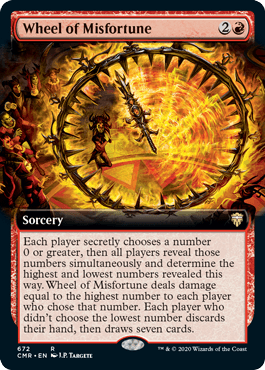
\includegraphics[width=0.1\textwidth]{wheel.jpg}  \\
\end{center}
\textbf{O Mestre (Game Master):} Um engenheiro sênior que conhece bem o sistema.  
Ele escolhe um incidente que já aconteceu de verdade (baseado em um Postmortem antigo).

\vspace{0.3cm}
\textbf{O Jogador:} Um engenheiro (geralmente alguém entrando no rodízio de plantão/on-call).

\vspace{0.3cm}
\textbf{O Cenário:} 
\begin{itemize}
    \item Mestre diz: "São 3 da manhã, seu Pager toca."
    \item Alerta: Latência no Checkout acima de 500ms.
    \item Pergunta ao jogador: "O que você faz?"
\end{itemize}
\end{frame}

% Slide 2
\begin{frame}{2. O Encaixe nas Boas Práticas do Google}
\textbf{A. Validação dos Manuais de Plantão (Playbooks)}
\begin{itemize}
    \item Se o jogador diz "Vou olhar o manual" e ele estiver desatualizado ou confuso, o grupo descobre isso na simulação.
    \item Resultado: O time atualiza o manual imediatamente após o jogo.
\end{itemize}

\vspace{0.3cm}
\textbf{B. Redução da "Fadiga de Alerta"}
\begin{itemize}
    \item Durante o jogo, o mestre pode lançar alertas falsos (ruído).
    \item O jogador aprende a filtrar o que é crítico e o que é distração.
    \item Resultado: O time aprende a calibrar alertas para que sejam úteis, não irritantes.
\end{itemize}
\end{frame}
% ----------------------------------------------------------------
% SLIDE 5 — As coisas quebram; a vida é assim
% ----------------------------------------------------------------
\begin{frame}{5) As coisas quebram — a vida é assim}

  \begin{columns}[T]
    \column{0.50\textwidth}
      \begin{itemize}
        \item Falhas são \textbf{inevitáveis} em qualquer sistema ou empresa
        \item O que diferencia uma organização resiliente é \textbf{como as pessoas respondem}
        \item Uma boa resposta exige:
          \begin{itemize}
            \item \textbf{Preparação} antecipada
            \item \textbf{Treinamento} periódico, pertinente e prático
            \item \textbf{Suporte da diretoria e da gerência}
          \end{itemize}
        \item Investir em testes e treinamentos pode custar \textbf{dinheiro, tempo e até uptime} — e vale a pena
        \item Incidentes bem tratados viram \textbf{oportunidades de aprendizado} (postmortems)
      \end{itemize}

    \column{0.46\textwidth}
      \centering
      \begin{tikzpicture}[font=\small, scale=0.82, transform shape,
                          node distance=0.85cm]
        \tikzstyle{bloco}=[rectangle, rounded corners=4pt, draw=meuazul, thick,
                           fill=blue!10, minimum width=3.2cm,
                           minimum height=0.65cm, text centered]
        \tikzstyle{dest}=[rectangle, rounded corners=4pt, draw=meuverde, thick,
                          fill=green!12, minimum width=3.2cm,
                          minimum height=0.65cm, text centered]

        \node[bloco, fill=red!15, draw=meuvermelhoescuro] (falha)
          {Falha ocorre};
        \node[bloco, below=of falha] (prep) {Preparação prévia};
        \node[bloco, below=of prep] (trei) {Treinamento da equipe};
        \node[bloco, below=of trei] (supo) {Suporte da gestão};
        \node[dest, below=of supo] (resp) {Resposta eficiente};
        \node[dest, below=of resp] (apre) {Aprendizado (postmortem)};

        \foreach \a/\b in {falha/prep, prep/trei, trei/supo, supo/resp, resp/apre}
          \draw[->, thick, meuazul] (\a) -- (\b);
      \end{tikzpicture}
  \end{columns}
\end{frame}

% ----------------------------------------------------------------
% SLIDE 6 — O que fazer quando os sistemas falham
% ----------------------------------------------------------------
\begin{frame}{6) O que fazer quando os sistemas falham}

  \begin{columns}[T]
    \column{0.50\textwidth}
      \textbf{Protocolo básico de resposta:}
      \begin{itemize}
        \item \textbf{Não entre em pânico} — você foi treinado para isso
        \item Lembre-se: \textit{raramente há risco físico}; mantenha a calma
        \item \textbf{Avalie o escopo} do problema antes de agir
        \item Se sentir sobrecarregado: \textbf{chame mais pessoas}
          \begin{itemize}
            \item Page para o time ou para toda a empresa se necessário
          \end{itemize}
        \item Siga o \textbf{processo de resposta a incidentes} da empresa. Documente as ações tomadas para o \textbf{postmortem}
        
      \end{itemize}

    \column{0.46\textwidth}
      \centering
      \begin{tikzpicture}[font=\small, scale=0.85, transform shape,
                          node distance=0.5cm and 1.8cm]
        \tikzstyle{dec}=[diamond, draw=meuazul, thick, fill=blue!10,
                         minimum width=2.6cm, minimum height=0.8cm,
                         text centered, aspect=2]
        \tikzstyle{ac}=[rectangle, rounded corners=3pt, draw=meuazul, thick,
                        fill=blue!10, minimum width=2.8cm,
                        minimum height=0.6cm, text centered]
        \tikzstyle{ok}=[rectangle, rounded corners=3pt, draw=meuverde, thick,
                        fill=green!12, minimum width=2.8cm,
                        minimum height=0.6cm, text centered]

        \node[ac, fill=red!15, draw=meuvermelhoescuro] (inc) {Incidente};
        \node[ac, below=of inc] (calma) {Manter calma};
        \node[dec, below=of calma] (sozinho) {Sobrecarregado?};
        \node[ac, right=0.6cm of sozinho, yshift=-1.1cm,
              fill=orange!15, draw=orange!70!black] (page) {Chamar reforços};
        \node[ac, below=1.8cm of sozinho] (proc) {Seguir processo de incidentes};
        \node[ok, below=of proc] (post) {Postmortem e aprendizado};

        \draw[->, thick, meuazul] (inc) -- (calma);
        \draw[->, thick, meuazul] (calma) -- (sozinho);
        \draw[->, thick, orange!70!black]
          (sozinho) -- node[above, font=\scriptsize]{Sim} (page);
        \draw[->, thick, meuazul]
          (sozinho) -- node[left, font=\scriptsize]{Não} (proc);
        \draw[->, thick, orange!70!black] (page) |- (proc);
        \draw[->, thick, meuazul] (proc) -- (post);
      \end{tikzpicture}
  \end{columns}
\end{frame}

% ----------------------------------------------------------------
% SLIDE 7 — Emergência induzida por testes
% ----------------------------------------------------------------
\begin{frame}{7) Emergência Induzida por Testes}

  \begin{columns}[T]
    \column{1\textwidth}
      \begin{itemize}
        \item O Google adota uma abordagem \textbf{proativa}: provocar falhas de forma controlada
        \item Objetivo: observar como os sistemas falham e \textbf{melhorar a confiabilidade}
        \item Na maioria das vezes as falhas controladas ocorrem \textbf{conforme planejado}:
          \begin{itemize}
            \item Sistemas se comportam como esperado
            \item Dependências ocultas são reveladas
            \item Ações de \textit{follow-up} são documentadas
          \end{itemize}
        \item Às vezes os resultados \textbf{divergem drasticamente} das suposições
        \item Esses casos são os mais valiosos para o aprendizado
      \end{itemize}


  \end{columns}
\end{frame}
\begin{frame}{8) Emergência Induzida por Testes}

      \begin{tikzpicture}[font=\small, scale=0.82, transform shape,
                          node distance=0.5cm]
        \tikzstyle{bloco}=[rectangle, rounded corners=4pt, draw=meuazul,
                           thick, fill=blue!10, minimum width=2.2cm,
                           minimum height=0.65cm, text centered]
        \tikzstyle{bom}=[rectangle, rounded corners=4pt, draw=meuverde,
                         thick, fill=green!12, minimum width=3.2cm,
                         minimum height=0.65cm, text centered]
        \tikzstyle{ruim}=[rectangle, rounded corners=4pt,
                          draw=meuvermelhoescuro, thick, fill=red!10,
                          minimum width=3.2cm, minimum height=0.45cm,
                          text centered]

        \node[bloco] (plan) {Planejar teste};
        \node[bloco, below=of plan] (exec) {Executar falha controlada};
        \node[bloco, below=of exec, draw=orange!70!black, fill=orange!10]
          (obs) {Observar comportamento};

        % Dois caminhos
        \node[bom, below left=0.9cm and 0cm of obs] (ok)
          {Conforme esperado};
        \node[ruim, below right=0.9cm and 0.2cm of obs] (diver)
          {Resultado divergente};

        \node[bom, below=2.2cm of obs] (doc)
          {Documentar e corrigir};

        \draw[->, thick, meuazul] (plan) -- (exec);
        \draw[->, thick, meuazul] (exec) -- (obs);
        \draw[->, thick, meuverde] (obs) -| (ok);
        \draw[->, thick, meuvermelhoescuro] (obs) -| (diver);
        \draw[->, thick, meuverde] (ok) |- (doc);
        \draw[->, thick, meuvermelhoescuro] (diver) |- (doc);
      \end{tikzpicture}
\end{frame}

% ----------------------------------------------------------------
% SLIDE 8 — Caso: teste no MySQL
% ----------------------------------------------------------------
\begin{frame}{8) Estudo de Caso — Teste no MySQL}

  \begin{columns}[T]
    \column{0.6\textwidth}
      \textbf{Detalhes do teste:}
      \begin{itemize}
        \item Alvo: um dos maiores bancos de dados MySQL distribuídos do Google
        \item Plano: bloquear acesso a \textbf{1 banco entre 100}
        \item Objetivo: revelar \textbf{dependências ocultas}
      \end{itemize}
      \textbf{O que aconteceu:}
      \begin{itemize}
        \item Minutos após o início: múltiplos serviços externos e internos \textbf{ficaram inacessíveis}
        \item Sistemas em estado \textbf{intermitente ou parcialmente disponíveis}
        \item SRE abortou imediatamente o teste
        \item \textit{Rollback} das permissões não funcionou de imediato. Acesso totalmente restaurado \textbf{em 1 hora} via abordagem alternativa
      \end{itemize}

    \column{0.36\textwidth}
      \centering
      \begin{tikzpicture}[font=\scriptsize, scale=0.80, transform shape,
                          node distance=0.65cm and 0.5cm]
        \tikzstyle{ev}=[rectangle, rounded corners=3pt, draw=meuazul, thick,
                        fill=blue!10, minimum width=3.4cm,
                        minimum height=0.6cm, text centered]
        \tikzstyle{alerta}=[rectangle, rounded corners=3pt,
                            draw=meuvermelhoescuro, thick, fill=red!10,
                            minimum width=3.4cm, minimum height=0.6cm,
                            text centered]
        \tikzstyle{ok}=[rectangle, rounded corners=3pt, draw=meuverde, thick,
                        fill=green!12, minimum width=3.4cm,
                        minimum height=0.6cm, text centered]

        \node[ev] (t0) {Início do teste};
        \node[alerta, below=of t0] (t1) {Serviços reportam falhas};
        \node[alerta, below=of t1] (t2) {Teste abortado};
        \node[alerta, below=of t2] (t3) {Rollback falha};
        \node[ev, below=of t3] (t4) {Brainstorming de restauração};
        \node[ev, below=of t4] (t5) {Fix paralelo nas libs};
        \node[ok, below=of t5] (t6) {Acesso restaurado (1h)};

        \foreach \a/\b in {t0/t1,t1/t2,t2/t3,t3/t4,t4/t5,t5/t6}
          \draw[->, thick, meuazul] (\a) -- (\b);

        % Tempo
        \node[right=0.1cm of t0, meucinza] {t=0 min};
        \node[right=0.1cm of t6, meucinza] {t=60 min};
      \end{tikzpicture}
  \end{columns}
\end{frame}

% ----------------------------------------------------------------
% SLIDE 9 — Descobertas e lições aprendidas
% ----------------------------------------------------------------
\begin{frame}{9) Descobertas e Lições Aprendidas}

  \begin{columns}[T]
    \column{\textwidth}
      \textbf{O que deu certo:}
      \begin{itemize}
        \item Serviços afetados \textbf{escalaram imediatamente} o problema
        \item Equipe abortou o teste \textbf{sem entrar em pânico}
        \item Esforços \textbf{paralelos} aceleraram a restauração
        \item Ações corretivas foram \textbf{rápidas e completas}
      \end{itemize}
      \vspace{0.4em}
      \textbf{O que aprendemos:}
      \begin{itemize}
        \item Compreensão \textbf{insuficiente} das dependências entre sistemas
        \item Processo de resposta a incidentes \textbf{não havia sido comunicado} a todos
        \item Procedimentos de \textit{rollback} \textbf{devem ser testados} antes de testes em larga escala
        \item Testes periódicos são essenciais para \textbf{evitar reincidências}
      \end{itemize}

    
  \end{columns}
\end{frame}

% ----------------------------------------------------------------
% SLIDE 10 — Emergência induzida por alterações: visão geral
% ----------------------------------------------------------------
\begin{frame}{10) Emergência Induzida por Alterações}

  \begin{columns}[T]
    \column{0.70\textwidth}
      \begin{itemize}
        \item O Google realiza \textbf{inúmeros testes} em mudanças de configuração
        \item A escala e complexidade tornam \textbf{impossível prever} todas as dependências
        \item \textbf{Detalhes do caso:}
          \begin{itemize}
            \item Mudança de configuração em infraestrutura de \textbf{proteção contra abusos}
            \item Implantada globalmente em uma \textbf{sexta-feira}
            \item Disparou um bug que causou \textbf{falhas sucessivas} em toda a frota
            \item Serviços internos e externos ficaram simultaneamente indisponíveis
          \end{itemize}
        \item A infraestrutura interna também depende dos próprios serviços do Google — o impacto foi \textbf{cascata}
      \end{itemize}

    \column{0.26\textwidth}
      \centering
      \begin{tikzpicture}[font=\small, scale=0.80, transform shape,
                          node distance=0.75cm]
        \tikzstyle{bloco}=[rectangle, rounded corners=4pt, draw=meuazul, thick,
                           fill=blue!10, minimum width=3.3cm,
                           minimum height=0.65cm, text centered]
        \tikzstyle{ruim}=[rectangle, rounded corners=4pt,
                          draw=meuvermelhoescuro, thick, fill=red!10,
                          minimum width=3.3cm, minimum height=0.65cm,
                          text centered]

        \node[bloco] (conf) {Mudança de configuração};
        \node[ruim, below=of conf] (bug) {Bug acionado};
        \node[ruim, below=of bug] (frota) {Falhas em toda a frota};
        \node[ruim, below=of frota] (ext) {Serviços externos offline};
        \node[ruim, below=of ext] (int) {Serviços internos offline};

        \foreach \a/\b in {conf/bug,bug/frota,frota/ext,ext/int}
          \draw[->, thick, meuvermelhoescuro] (\a) -- (\b);

        % Rótulo
        \node[right=0.05cm of conf, font=\scriptsize, meucinza] {t=0};
        \node[right=0.05cm of int, font=\scriptsize, meucinza] {cascata};
      \end{tikzpicture}
  \end{columns}
\end{frame}

% ----------------------------------------------------------------
% SLIDE 11 — Resposta ao incidente de configuração
% ----------------------------------------------------------------
\begin{frame}{11) Resposta — Incidente de Configuração}

  \begin{columns}[T]
    \column{0.70\textwidth}
      \begin{itemize}
        \item \textbf{Segundos após a mudança:} alertas de monitoração dispararam
        \item Engenheiros de plantão migraram para \textbf{salas de segurança} (quartos de pânico) com acesso de backup à produção
        \item \textbf{5 minutos após:} engenheiro responsável fez \textbf{rollback} da mudança ao tomar conhecimento da falha corporativa
        \item Serviços começaram a se recuperar logo após o rollback
        \item \textbf{10 minutos após:} incidente declarado formalmente; procedimentos internos acionados
        \item Alguns serviços com bugs não relacionados só se recuperaram \textbf{após 1 hora}
      \end{itemize}

    \column{0.26\textwidth}
      \centering
      \begin{tikzpicture}[font=\scriptsize, scale=0.82, transform shape,
                          node distance=0.60cm]
        \tikzstyle{ev}=[rectangle, rounded corners=3pt, draw=meuazul, thick,
                        fill=blue!10, minimum width=3.4cm,
                        minimum height=0.6cm, text centered]
        \tikzstyle{alerta}=[rectangle, rounded corners=3pt,
                            draw=meuvermelhoescuro, thick, fill=red!10,
                            minimum width=3.4cm, minimum height=0.6cm,
                            text centered]
        \tikzstyle{ok}=[rectangle, rounded corners=3pt, draw=meuverde, thick,
                        fill=green!12, minimum width=3.4cm,
                        minimum height=0.6cm, text centered]

        \node[ev] (t0) {Mudança implantada};
        \node[alerta, below=of t0] (t1) {Alertas disparam (segundos)};
        \node[alerta, below=of t1] (t2) {Engenheiros vão p/ sala segura};
        \node[ok, below=of t2] (t3) {Rollback feito (5 min)};
        \node[ev, below=of t3] (t4) {Incidente declarado (10 min)};
        \node[ok, below=of t4] (t5) {Recuperação completa (1h)};

        \foreach \a/\b in {t0/t1,t1/t2,t2/t3,t3/t4,t4/t5}
          \draw[->, thick, meuazul] (\a) -- (\b);

        \node[right=0.1cm of t0, meucinza] {t=0};
        \node[right=0.1cm of t5, meucinza] {t=60 min};
      \end{tikzpicture}
  \end{columns}
\end{frame}

% ----------------------------------------------------------------
% SLIDE 12 — Descobertas e lições: mudanças de configuração
% ----------------------------------------------------------------
\begin{frame}{12) Descobertas e Lições — Mudanças de Configuração}

  \begin{columns}[T]
    \column{0.65\textwidth}
    \small  
    \textbf{O que deu certo:}
      \begin{itemize}
        \item Monitoração detectou o problema \textbf{quase imediatamente}
        \item Sistemas de comunicação em \textbf{banda alternativa} mantiveram a equipe conectada
        \item Ferramentas de \textbf{linha de comando} e acesso alternativo permitiram o rollback
        \item Infraestrutura \textbf{limitou a velocidade} de propagação das falhas (throttling)
      \end{itemize}
      

    \column{0.36\textwidth}
      \centering
      \begin{tikzpicture}[font=\scriptsize, scale=0.82, transform shape]
        \tikzstyle{tit}=[font=\small\bfseries, align=center]
        \tikzstyle{item}=[font=\scriptsize, align=left, text width=2.8cm]

        % Certo
        \node[rectangle, draw=meuverde, thick, fill=green!10,
              minimum width=3.3cm, minimum height=4.0cm, anchor=north west]
          at (0,0) {};
        \node[tit, text=meuverde] at (1.65,-0.35) {Positivo};
        \node[item] at (1.65,-1.55)
          {Monitoração rápida\\Comm. alternativa\\Rollback disponível\\Throttling de falhas\\Sorte (diligência)};

        % Aprendido
        \node[rectangle, draw=meuvermelhoescuro, thick, fill=red!10,
              minimum width=3.3cm, minimum height=4.0cm, anchor=north west]
          at (3.6,0) {};
        \node[tit, text=meuvermelhoescuro] at (5.25,-0.35) {A melhorar};
        \node[item] at (5.25,-1.55)
          {Canary rigoroso\\Alertas calibrados\\Treinar ferramentas\\Reduzir depend. internas};
      \end{tikzpicture}
  \end{columns}
\end{frame}
\begin{frame}{12) Descobertas e Lições — Mudanças de Configuração}

  \begin{columns}[T]
    \column{0.65\textwidth}
    \small  
    \textbf{O que aprendemos:}
      \begin{itemize}
        \item \textbf{Canary incompleto} — palavra-chave rara não foi exercitada
        \item Mudanças percebidas como ``de baixo risco'' também precisam de \textbf{canary rigoroso}
        \item Alertas excessivos \textbf{sobrecarregaram} os engenheiros de plantão
        \item Equipe precisava de \textbf{maior familiaridade} com ferramentas de backup
        \item Dependência das próprias ferramentas internas agravaria uma interrupção mais longa
      \end{itemize}------
      

    \column{0.36\textwidth}
      \centering
      \begin{tikzpicture}[font=\scriptsize, scale=0.82, transform shape]
        \tikzstyle{tit}=[font=\small\bfseries, align=center]
        \tikzstyle{item}=[font=\scriptsize, align=left, text width=2.8cm]

        % Certo
        \node[rectangle, draw=meuverde, thick, fill=green!10,
              minimum width=3.3cm, minimum height=4.0cm, anchor=north west]
          at (0,0) {};
        \node[tit, text=meuverde] at (1.65,-0.35) {Positivo};
        \node[item] at (1.65,-1.55)
          {Monitoração rápida\\Comm. alternativa\\Rollback disponível\\Throttling de falhas\\Sorte (diligência)};

        % Aprendido
        \node[rectangle, draw=meuvermelhoescuro, thick, fill=red!10,
              minimum width=3.3cm, minimum height=4.0cm, anchor=north west]
          at (3.6,0) {};
        \node[tit, text=meuvermelhoescuro] at (5.25,-0.35) {A melhorar};
        \node[item] at (5.25,-1.55)
          {Canary rigoroso\\Alertas calibrados\\Treinar ferramentas\\Reduzir depend. internas};
      \end{tikzpicture}
  \end{columns}
\end{frame}
% ----------------------------------------------------------------
% SLIDE 13 — Emergência induzida por processo: detalhes
% ----------------------------------------------------------------
\begin{frame}{13) Emergência Induzida por Processo}

  \begin{columns}[T]
    \column{0.55\textwidth}
      \begin{itemize}
        \item A automação do Google é poderosa — e, às vezes, \textbf{rápida demais}
        \item \textbf{Detalhes do caso:}
          \begin{itemize}
            \item Duas requisições consecutivas de \textbf{desativação} foram enviadas para a mesma instalação
            \item Um \textbf{bug sutil} na automação interpretou resposta vazia como ``\textit{todas as máquinas}''
            \item Resultado: todas as máquinas enviadas para a fila do \textbf{Diskerase} globalmente
            \item Discos rígidos limpos; máquinas incapazes de responder a requisições
          \end{itemize}
        \item \textbf{Lição central:} \textit{zero} pode significar \textit{tudo} — verificações de sanidade são essenciais
      \end{itemize}

    \column{0.42\textwidth}
      \centering
      \begin{tikzpicture}[font=\scriptsize, scale=0.82, transform shape,
                          node distance=0.62cm]
        \tikzstyle{ev}=[rectangle, rounded corners=3pt, draw=meuazul, thick,
                        fill=blue!10, minimum width=3.5cm,
                        minimum height=0.62cm, text centered]
        \tikzstyle{ruim}=[rectangle, rounded corners=3pt,
                          draw=meuvermelhoescuro, thick, fill=red!10,
                          minimum width=3.5cm, minimum height=0.62cm,
                          text centered]

        \node[ev] (r1) {Requisição de desativação \#1};
        \node[ev, below=of r1] (r2) {Requisição de desativação \#2};
        \node[ruim, below=of r2] (bug) {Bug: filtro vazio = todas};
        \node[ruim, below=of bug] (disk) {Diskerase global};
        \node[ruim, below=of disk] (off) {Máquinas offline};
        \node[ruim, below=of off] (req) {Falhas em requisições};

        \foreach \a/\b in {r1/r2,r2/bug,bug/disk,disk/off,off/req}
          \draw[->, thick, meuvermelhoescuro] (\a) -- (\b);
      \end{tikzpicture}
  \end{columns}
\end{frame}

% ----------------------------------------------------------------
% SLIDE 14 — Resposta e recuperação do incidente de processo
% ----------------------------------------------------------------
\begin{frame}{14) Resposta e Recuperação — Incidente de Processo}

  \begin{columns}[T]
    \column{0.75\textwidth}
     \small
      \textbf{Resposta imediata:}
      \begin{itemize}
        \item Page acionado; engenheiros \textbf{drenaram o tráfego} das localidades afetadas
        \item Tráfego redirecionado para instalações maiores (não afetadas)
        \item \textbf{Toda a automação da equipe foi desabilitada} para evitar mais danos
        \item Em \textbf{1 hora}: tráfego completamente desviado; interrupção superada
      \end{itemize}
      \vspace{0.3em}
      \textbf{Recuperação (a parte difícil):}
      \begin{itemize}
        \item Congestionamentos de rede tratados em paralelo
        \item Primeira instalação reconstruída em \textbf{3 horas}
        \item Equipe dividida em 3 grupos com etapas definidas de reinstalação
        \item \textbf{Maioria da capacidade} restaurada em 3 dias; retardatários em 1–2 meses
      \end{itemize}

    \column{0.28\textwidth}
      \centering
      \begin{tikzpicture}[font=\scriptsize, scale=0.80, transform shape,
                          node distance=0.58cm]
        \tikzstyle{ok}=[rectangle, rounded corners=3pt, draw=meuverde, thick,
                        fill=green!12, minimum width=3.5cm,
                        minimum height=0.60cm, text centered]
        \tikzstyle{ev}=[rectangle, rounded corners=3pt, draw=meuazul, thick,
                        fill=blue!10, minimum width=3.5cm,
                        minimum height=0.60cm, text centered]

        \node[ev] (p) {Page recebido};
        \node[ok, below=of p] (dr) {Tráfego drenado};
        \node[ok, below=of dr] (at) {Automação desabilitada};
        \node[ok, below=of at] (1h) {Interrupção superada (1h)};
        \node[ev, below=of 1h] (rec) {Início da recuperação};
        \node[ok, below=of rec] (3h) {1ª instalação online (3h)};
        \node[ok, below=of 3h] (3d) {Capacidade majoritária (3d)};

        \foreach \a/\b in {p/dr,dr/at,at/1h,1h/rec,rec/3h,3h/3d}
          \draw[->, thick, meuazul] (\a) -- (\b);

        \node[right=0.05cm of p, meucinza] {t=0};
        \node[right=0.05cm of 3d, meucinza] {t=3d};
      \end{tikzpicture}
  \end{columns}
\end{frame}

% ----------------------------------------------------------------
% SLIDE 15 — Lições e conclusão
% ----------------------------------------------------------------
\begin{frame}{15) Todos os Problemas Têm Soluções}

  \begin{columns}[T]
    \column{0.55\textwidth}
      \textbf{O que deu certo:}
      \begin{itemize}
        \item Instalações \textbf{grandes} não foram afetadas (arquitetura diferente)
        \item Transferência rápida de tráfego; usuários atendidos com latência mínima
        \item Protocolos de resposta a incidentes \textbf{maduros} e bem executados
        \item Colaboração exemplar entre equipes e geografias
      \end{itemize}
      \vspace{0.3em}
    \column{0.42\textwidth}
      \centering
      \begin{tikzpicture}[font=\small, scale=0.80, transform shape]
        % Círculo central
        \node[circle, draw=meuazul, thick, fill=blue!15,
              minimum size=2.0cm, align=center] (c) at (0,0)
          {Todo\\problema\\tem\\solução};

        % Satélites
        \foreach \ang/\lab/\col in {
          90/{Resposta\\rápida}/meuverde,
          162/{Colaboração\\entre times}/meuazul,
          234/{Verificações\\de sanidade}/meuvermelhoescuro,
          306/{Processos\\maduros}/meucinza,
          18/{Registrar e\\aprender}/meuverde}{
          \node[rectangle, rounded corners=3pt, draw=\col, thick,
                fill=\col!10, minimum width=1.9cm, minimum height=0.8cm,
                text centered, font=\scriptsize, align=center]
            (\ang) at (\ang:3.0cm) {\lab};
          \draw[->, thick, \col] (c) -- (\ang);
        }
      \end{tikzpicture}
  \end{columns}
\end{frame}
\begin{frame}{15) Todos os Problemas Têm Soluções}

  \begin{columns}[T]
    \column{0.55\textwidth}
      \textbf{O que aprendemos:}
      \begin{itemize}
        \item Automação precisa de \textbf{verificações de sanidade} — zero $\neq$ ``sem filtro''
        \item Reinstalação via \textbf{TFTP com QoS baixo} é lenta e não confiável em escala
        \item Infraestrutura de reinstalação deve \textbf{suportar cargas excepcionais}
        \item \textbf{Envolva quem disparou o evento} — é quem mais sabe do estado atual
        \item Após a crise: \textbf{registre, limpe e aprenda}
      \end{itemize}

    \column{0.42\textwidth}
      \centering
      \begin{tikzpicture}[font=\small, scale=0.80, transform shape]
        % Círculo central
        \node[circle, draw=meuazul, thick, fill=blue!15,
              minimum size=2.0cm, align=center] (c) at (0,0)
          {Todo\\problema\\tem\\solução};

        % Satélites
        \foreach \ang/\lab/\col in {
          90/{Resposta\\rápida}/meuverde,
          162/{Colaboração\\entre times}/meuazul,
          234/{Verificações\\de sanidade}/meuvermelhoescuro,
          306/{Processos\\maduros}/meucinza,
          18/{Registrar e\\aprender}/meuverde}{
          \node[rectangle, rounded corners=3pt, draw=\col, thick,
                fill=\col!10, minimum width=1.9cm, minimum height=0.8cm,
                text centered, font=\scriptsize, align=center]
            (\ang) at (\ang:3.0cm) {\lab};
          \draw[->, thick, \col] (c) -- (\ang);
        }
      \end{tikzpicture}
  \end{columns}
\end{frame}


% ----------------------------------------------------------------
% SLIDE 16 — Mantenha um histórico: postmortems
% ----------------------------------------------------------------
\begin{frame}{16) Aprenda com o Passado — Postmortems}

  \begin{columns}[T]
    \column{0.52\textwidth}
      \begin{itemize}
        \item \textbf{Documente} cada interrupção de serviço com honestidade
        \item Postmortems eficazes respondem:
          \begin{itemize}
            \item \textit{O que falhou?} (causa-raiz)
            \item \textit{Como evitar?} (tático e estratégico)
            \item \textit{Quem é responsável pelo follow-up?}
          \end{itemize}
        \item \textbf{Publique e organize} os postmortems — a história é de todos
        \item \textbf{Atribua responsabilidades} e acompanhe as ações corretivas
        \item Um bom histórico evita que a \textbf{mesma interrupção aconteça duas vezes}
      \end{itemize}

    \column{0.45\textwidth}
      \centering
      \begin{tikzpicture}[font=\small, scale=0.88, transform shape,
                          node distance=1.0cm]
        % Ciclo de melhoria contínua
        \tikzstyle{fase}=[rectangle, rounded corners=5pt, draw=meuazul, thick,
                          fill=blue!10, minimum width=2.8cm,
                          minimum height=0.7cm, text centered]

        \node[fase, fill=red!15, draw=meuvermelhoescuro] (inc) {Incidente};
        \node[fase, right=1.2cm of inc] (post) {Postmortem};
        \node[fase, below=0.9cm of post] (acao) {Ações corretivas};
        \node[fase, below=0.9cm of inc, fill=green!12, draw=meuverde]
          (melhora) {Sistema mais robusto};

        \draw[->, thick, meuvermelhoescuro] (inc) -- (post);
        \draw[->, thick, meuazul] (post) -- (acao);
        \draw[->, thick, meuverde] (acao) -- (melhora);
        \draw[->, thick, meuazul, dashed] (melhora) -- (inc)
          node[midway, left, font=\scriptsize]{ciclo};

        % Rótulos
        \node[font=\scriptsize, meucinza, below=0.1cm of post]
          {\textit{honesto e completo}};
        \node[font=\scriptsize, meucinza, below=0.1cm of acao]
          {\textit{com responsáveis}};
      \end{tikzpicture}
  \end{columns}
\end{frame}

% ----------------------------------------------------------------
% SLIDE 17 — Faça as perguntas "E se...?" e incentive testes proativos
% ----------------------------------------------------------------
\begin{frame}{17) Perguntas Difíceis e Testes Proativos}

  \begin{columns}[T]
    \column{0.50\textwidth}
     \small
      \textbf{Faça as perguntas ``E se\ldots?'':}
      \begin{itemize}
        \item E se a \textbf{energia do prédio cair}?
        \item E se o \textbf{datacenter ficar às escuras}?
        \item E se alguém \textbf{comprometer seu servidor web}?
        \item Você tem um \textbf{plano}? Você sabe como \textbf{reagir}?
        \item A pessoa ao seu lado poderia fazer o mesmo?
      \end{itemize}
      \textbf{Incentive testes proativos:}
      \begin{itemize}
        \item \textbf{Teoria $\neq$ realidade} — só testando você saberá
        \item Prefira que a falha ocorra durante um \textbf{teste supervisionado} a às 2h da manhã sem aviso e não conte com suposições não verificadas
      \end{itemize}

    \column{0.47\textwidth}
      \centering
      \begin{tikzpicture}[font=\small, scale=0.82, transform shape]
        % Dois retângulos: teoria vs realidade
        \tikzstyle{caixa}=[rectangle, rounded corners=4pt, thick,
                           minimum width=3.0cm, minimum height=1.0cm,
                           text centered]

        \node[caixa, draw=meuazul, fill=blue!10] (teo) at (0,0) {Teoria};
        \node[caixa, draw=meuvermelhoescuro, fill=red!10] (rea) at (4.0,0)
          {Realidade};

        \draw[<->, very thick, orange!80!black] (teo) -- (rea)
          node[midway, above, font=\scriptsize]{$\neq$}
          node[midway, below, font=\scriptsize]{teste proativo};

        % Exemplos "E se" abaixo
        \foreach \y/\txt in {
          -1.3/{E se a energia cair?},
          -2.0/{E se o datacenter apagar?},
          -2.7/{E se o servidor for comprometido?},
          -3.4/{Você tem um plano?}}{
          \node[draw=meucinza, rounded corners=2pt, fill=gray!8,
                font=\scriptsize, minimum width=5.5cm,
                minimum height=0.5cm, text centered] at (2.0,\y) {\txt};
        }
      \end{tikzpicture}
  \end{columns}
\end{frame}
% ----------------------------------------------------------------
% SLIDE 18 — Conclusão: o ciclo que nunca para
% ----------------------------------------------------------------
\begin{frame}{18) Conclusão — O Ciclo de Melhoria Contínua}

  \begin{columns}[T]
    \column{0.52\textwidth}
      \begin{itemize}
        \item Três emergências, três origens diferentes:
          \begin{itemize}
            \item \textbf{Teste proativo} (MySQL)
            \item \textbf{Mudança de configuração} (bug de canary)
            \item \textbf{Automação de desativação} (Diskerase)
          \end{itemize}
        \item Mas as \textbf{respostas tiveram muito em comum}:
          \begin{itemize}
            \item Sem pânico
            \item Convocação de mais pessoas
            \item Aprendizado com o passado
            \item Documentação e follow-up
            \item Testes proativos subsequentes
          \end{itemize}
        \item O ciclo é \textbf{universal} — aplica-se a qualquer empresa, de qualquer porte
      \end{itemize}

    \column{0.45\textwidth}
      \centering
      \begin{tikzpicture}[font=\scriptsize, scale=0.90, transform shape]
        % Triângulo de melhoria
        \coordinate (A) at (0,0);
        \coordinate (B) at (3.5,0);
        \coordinate (C) at (1.75,3.0);

        \draw[thick, meuazul, fill=blue!5] (A) -- (B) -- (C) -- cycle;

        % Nodes nos vértices
        \node[draw=meuvermelhoescuro, fill=red!10, rounded corners=3pt,
              minimum width=2.0cm, minimum height=0.65cm, text centered]
              at (A) {Incidente};

        \node[draw=meuazul, fill=blue!10, rounded corners=3pt,
              minimum width=2.0cm, minimum height=0.65cm, text centered]
              at (B) {Postmortem};

        \node[draw=meuverde, fill=green!10, rounded corners=3pt,
              minimum width=2.2cm, minimum height=0.65cm, text centered]
              at (C) {Sistema robusto};

        % Setas nas arestas
        \draw[->, thick, meuvermelhoescuro] (0.6,0.15) -- (1.1,0.15); % A -> B (horizontal)
        \draw[->, thick, meuazul] (2.8,0.15) to[bend left=20] node[midway, right, font=\scriptsize]{aprender} (2.2,2.6); % B -> C
        \draw[->, thick, meuverde] (1.35,2.6) to[bend left=20] node[midway, left, font=\scriptsize]{testar} (0.5,0.2); % C -> A

        % Texto central
        \node[font=\small\bfseries, meucinza] at (1.75,1.0)
              {melhoria contínua};
      \end{tikzpicture}
  \end{columns}
\end{frame}

% ----------------------------------------------------------------
% Slide de encerramento
% ----------------------------------------------------------------
\begin{frame}
  \centering
  \Huge Obrigado!\\
  \vspace{1cm}
  \large Dúvidas?
\end{frame}

\end{document}
